\documentclass[11pt,oneside]{article}

\usepackage[T1]{fontenc}
\usepackage[utf8]{inputenc}
\IfFileExists{libertinus.sty}{\usepackage{libertinus}}{\usepackage{lmodern}}
\usepackage[a4paper,margin=25mm,headheight=15pt]{geometry}
\usepackage{microtype}
\usepackage{amsmath,amssymb,amsthm,mathtools,mathrsfs,bm}
\usepackage{booktabs,longtable,tabularx,array}
\usepackage{graphicx}
\usepackage{xcolor}
\usepackage{enumitem}
\usepackage{fancyhdr}
\usepackage{titlesec}
\usepackage{xurl}
\usepackage{listings}
\usepackage{float}
\usepackage[font=small,labelfont=bf]{caption}
\usepackage[hypertexnames=false]{hyperref}
\usepackage[nameinlink,noabbrev]{cleveref}

\graphicspath{{figures/}}
\definecolor{linkblue}{RGB}{27,73,125}
\definecolor{shadegray}{RGB}{246,247,249}
\definecolor{rulegray}{RGB}{195,201,208}
\hypersetup{
  colorlinks=true,
  linkcolor=linkblue,
  citecolor=linkblue,
  urlcolor=linkblue,
  pdftitle={Automatic Scale Factorizations of the Rvachev Law},
  pdfauthor={OpenAI GPT-5.6 Pro},
  pdfsubject={Thue-Morse scale splitting, Fabius and Rvachev functions, q-Mahler cocycles, Mellin transforms, small-ball asymptotics},
  pdfkeywords={Fabius, Rvachev, up-function, Thue-Morse, q-analog, sinc product, Mellin transform, Bernoulli, Bell, Lambert W, Legendre}
}

\pagestyle{fancy}
\fancyhf{}
\fancyhead[L]{\small Automatic scale factorizations}
\fancyhead[R]{\small\nouppercase{\leftmark}}
\fancyfoot[C]{\thepage}
\renewcommand{\headrulewidth}{0.4pt}
\titleformat{\section}{\Large\bfseries}{\thesection}{0.7em}{}
\titleformat{\subsection}{\large\bfseries}{\thesubsection}{0.7em}{}
\setcounter{secnumdepth}{3}
\setcounter{tocdepth}{2}
\setlist[itemize]{leftmargin=2em,itemsep=0.25em,topsep=0.4em}
\setlist[enumerate]{leftmargin=2.3em,itemsep=0.25em,topsep=0.4em}
\setlength{\emergencystretch}{2em}
\allowdisplaybreaks
\numberwithin{equation}{section}

\newtheorem{theorem}{Theorem}[section]
\newtheorem{proposition}[theorem]{Proposition}
\newtheorem{lemma}[theorem]{Lemma}
\newtheorem{corollary}[theorem]{Corollary}
\newtheorem{identity}[theorem]{Identity}
\newtheorem{conjecture}[theorem]{Conjecture}
\newtheorem{problem}[theorem]{Problem}
\theoremstyle{definition}
\newtheorem{definition}[theorem]{Definition}
\newtheorem{example}[theorem]{Example}
\newtheorem{algorithm}[theorem]{Algorithm}
\theoremstyle{remark}
\newtheorem{remark}[theorem]{Remark}
\newtheorem{warning}[theorem]{Warning}

\newcommand{\R}{\mathbb R}
\newcommand{\C}{\mathbb C}
\newcommand{\N}{\mathbb N}
\newcommand{\Z}{\mathbb Z}
\newcommand{\e}{\mathrm e}
\newcommand{\ii}{\mathrm i}
\newcommand{\dd}{\,\mathrm d}
\newcommand{\eps}{\varepsilon}
\newcommand{\sinc}{\operatorname{sinc}}
\newcommand{\Up}{\operatorname{up}}
\newcommand{\supp}{\operatorname{supp}}
\newcommand{\Law}{\operatorname{Law}}
\newcommand{\Var}{\operatorname{Var}}
\newcommand{\ord}{\operatorname{ord}}
\newcommand{\Mell}{\mathcal M}
\newcommand{\Bell}{\mathcal B}
\newcommand{\bigO}{\mathcal O}
\newcommand{\smallo}{o}
\newcommand{\one}{\mathbf 1}
\newcommand{\abs}[1]{\left\lvert#1\right\rvert}
\newcommand{\norm}[1]{\left\lVert#1\right\rVert}
\newcommand{\set}[1]{\left\{#1\right\}}
\newcommand{\floor}[1]{\left\lfloor#1\right\rfloor}
\newcommand{\ceil}[1]{\left\lceil#1\right\rceil}
\newcommand{\repo}{\texttt{ProveIt}}

\newenvironment{statusbox}[1]{%
  \par\smallskip\noindent\begin{center}\begin{minipage}{0.94\textwidth}%
  \hrule\vspace{0.55em}\textbf{#1.}\ }{%
  \vspace{0.55em}\hrule\end{minipage}\end{center}\smallskip}

\lstdefinestyle{pythonstyle}{
  language=Python,
  basicstyle=\ttfamily\small,
  backgroundcolor=\color{shadegray},
  frame=single,
  rulecolor=\color{rulegray},
  columns=fullflexible,
  keepspaces=true,
  showstringspaces=false,
  breaklines=true
}

\title{\bfseries Automatic Scale Factorizations of the Rvachev Law\\[0.35em]
\large Thue--Morse convolution factors, $q$-Mahler cocycles, Mellin boundaries,\\
Bernoulli--Bell moments, exact plateaux, and inverse-edge laws}
\author{Research report prepared for the \repo\ Fabius-function project}
\date{30 August 2026}

\begin{document}
\maketitle

\begin{abstract}
Write the centered Rvachev random variable as the convergent series
\[
 X=\sum_{n\ge1}U_n,\qquad U_n\sim\operatorname{Unif}[-2^{-n},2^{-n}],
\]
with independent summands.  Its density is Rvachev's up-function and its characteristic
function is the familiar infinite sinc product.  This report introduces a complementary
pair of compactly supported probability laws by assigning the scale $2^{-n}$ according
to the Prouhet--Thue--Morse sign $e_{n-1}=(-1)^{s_2(n-1)}$:
\[
 X_+=\sum_{e_{n-1}=1}U_n,
 \qquad
 X_-=\sum_{e_{n-1}=-1}U_n.
\]
Their densities $u_\pm$ are $C^\infty$, nonnegative, and satisfy the exact factorization
\[
 u_+*u_-=\Up.
\]
This is not an algebraic splitting of a formal transform: both factors are genuine smooth
probability densities.  Their support radii are controlled by the Thue--Morse--Mahler
product
\[
 E(q)=\sum_{m\ge0}e_mq^m=\prod_{j\ge0}(1-q^{2^j}),
\qquad
 R_\pm=\frac12\pm\frac14E\!\left(\frac12\right).
\]
Unexpectedly, each factor has an exact central plateau.  One has
$u_+(x)=1$ for $|x|\le R_-$, while
$u_-(x)=2$ for $|x|\le E(1/2)/4$.  The first plateau contains the entire support of
$u_-$; this gives a direct convolutional explanation of the infinite-order flatness of
$\Up$ at the origin.

A complex parameter $q$ produces characteristic subproducts
\[
 \Phi_\sigma(z;q)=\prod_{m\ge0}
 \sinc(zq^{m+1})^{(1+\sigma e_m)/2},\qquad \sigma\in\{+1,-1\},
\]
which obey an exact two-component $q$-Mahler recursion.  Their logarithms have explicit
lacunary $q$-series, and all even cumulants are Bernoulli multiples of
\[
 \frac{q^{2r}}2\left(\frac1{1-q^{2r}}+\sigma E(q^{2r})\right).
\]
Consequently every moment is an explicit complete Bell polynomial, and every Legendre
coefficient is a finite expression in the same Mahler values.  The zero multiplicities
at $2\pi k$ are finite Thue--Morse prefix sums; they rule out nontrivial equal compactly
supported convolution roots of either factor as well as of the original Rvachev law.

For the signed log-moment correction we obtain the Mellin transform
\[
 \Mell J(s)=-\Gamma(s)\zeta(s+1)E(2^s),
 \qquad -2<\Re s<-1,
\]
and hence a natural boundary at $\Re s=0$.  The natural-boundary ingredient itself is
already occupied in the repository; its appearance here is recorded as a consequence
for the new factors, not as a new general theorem.  Finally, a selector-density theorem
gives sharp logarithmic edge asymptotics.  If a scale set has density $\delta$ and bounded
discrepancy, then
\[
 \log\Pr(R_A-X_A\le\eps)
 =-\frac{\delta}{2\log2}\left(\log\frac1\eps\right)^2
 +\bigO\!\left(\log\frac1\eps\log\log\frac1\eps\right).
\]
For both Thue--Morse factors $\delta=1/2$.  Inverting this law yields a new stretched
exponential endpoint scale for their quantile functions.  The report includes complete
proofs of the stated results, numerical verification, conjectural symbolic-hull refinements,
and a Lean formalization blueprint.
\end{abstract}

\begin{statusbox}{Status and originality convention}
Statements labelled theorem, proposition, lemma, corollary, or identity are proved below,
unless explicitly attributed to a cited source.  Conjectures and heuristic expansions are
visibly labelled.  ``New'' means apparently absent from the audited repository corpus; it
is not a claim of worldwide priority.  The arguments have not been peer reviewed or
machine checked.
\end{statusbox}

\tableofcontents
\clearpage

\section{Corpus audit and contribution boundary}
\label{sec:audit}

\subsection{How the source tree was read}

The requested directory is a living research corpus with current expositions, imported
papers, generated tables, formalization guides, large thematic volumes, and archived
pre-consolidation versions.  Counting every archived snapshot as an independent source
would exaggerate mathematical coverage while hiding the current source of record.  The
audit therefore used four complementary layers:
\begin{enumerate}
\item every visible \texttt{*.tex} path below
\path{Analysis/FabiusFunction/docs} was inventoried through the recursive GitHub tree and
the repository's generated manifests and corpus ledgers;
\item the primary Fabius--Rvachev exposition, glossary, Lean walkthrough, imported-paper
transcriptions, and current thematic frontiers were read at definition, theorem, and
open-problem level;
\item the closest-overlap reports were read in full or by their complete theorem summaries,
then searched for the proposed objects and formula patterns;
\item archived revisions were used as a provenance and duplication map, with consolidated
volumes treated as the active mathematical baseline.
\end{enumerate}
The companion file \texttt{NOVELTY\_AUDIT.md} records the targeted phrase and formula
searches.  The comparison was made against repository revision
\texttt{201f210d992878d66bea0e15eab5246e59355bed}, the revision surfaced by the recursive
source search on 30 August 2026.

\subsection{Occupied territory}

The corpus already develops, often in several generations, the following themes:
classical Fabius/Rvachev identities; exact dyadic values; Thue--Morse derivative signs;
infinite sinc products and Fourier decay; Bell and Bernoulli moment calculi; Legendre,
Lagrange, and Appell representations; dyadic and geometric comb interpolation; inverse
endpoint expansions with Lambert $W$; Borel singular lattices; q-Pochhammer and
q-binomial expansions; cyclotomic $q$-plane blow-ups; natural boundaries; spectral zeta
functions; total positivity; refinement operators; periodic polyphase factorizations by
residue classes of the scale index; and reciprocal-integer convolution divisors.  In
particular, the consolidated representation volume and the recent reports on cyclotomic
$q$-Fabius boundaries and quotients $\Phi(z)/\Phi(z/M)$ make it essential not to advertise
either generic natural boundaries or arbitrary convolution decompositions as new
\cite{RepresentationFrontiers,CyclotomicReport,DivisorReport}.  The present factors differ
from the occupied polyphase construction in that their scale selector is nonperiodic and
automatic rather than a residue class modulo a fixed integer.

The duplication search used such patterns as
\begin{center}
\begin{tabular}{llll}
\toprule
scale partition & selected dyadic scales & sinc subproduct & automatic factor\\
Thue--Morse selector & complementary factors & positive definite & exact plateau\\
$q$-Mahler pair & selector cumulants & support Mahler product & scale thinning\\
\bottomrule
\end{tabular}
\end{center}
No repository source found in that audit constructs the two probability laws studied here
by assigning the \emph{individual uniform summands} according to the two Thue--Morse
signs, nor the resulting plateau, zero-divisor, q-cumulant, and edge package.

\subsection{Result ledger}

The principal results distinct from the occupied baseline are:
\begin{enumerate}[label=\textbf{R\arabic*.},leftmargin=3.5em]
\item a general scale-subset factorization of the Rvachev law and its Thue--Morse pair;
\item exact support radii in terms of the Mahler product $E(1/2)$;
\item exact central plateaux and a convolutional proof of infinite-order flatness at the
origin of $\Up$;
\item an exact coupled $q$-Mahler recursion for the two characteristic factors;
\item closed Bernoulli cumulants, Bell moments, and finite Legendre coefficient formulae;
\item a Thue--Morse prefix formula for every real zero multiplicity;
\item obstruction to equal compactly supported convolution roots;
\item a Mellin transform whose signed part carries $E(2^s)$ and therefore the Thue--Morse
natural boundary;
\item a selector-density theorem for rapid Fourier decay, smoothness, small balls, and
inverse-edge quantiles;
\item finite dyadic spline approximants and an explicit route to certified computation;
\item conjectural shift-hull, Lambert-$W$, spectral-rigidity, and Jacobi-parameter frontiers.
\end{enumerate}

\section{Classical normalization: Fabius and Rvachev}
\label{sec:normalization}

Let $V_1,V_2,\ldots$ be independent random variables uniformly distributed on $[-1,1]$,
and define
\begin{equation}
 X=\sum_{n\ge1}2^{-n}V_n.
 \label{eq:full-random-series}
\end{equation}
The series converges absolutely almost surely, and $X$ is supported on $[-1,1]$.  In the
Fourier convention
\(
 \widehat f(z)=\int_\R \e^{\ii zx}f(x)\dd x
\)
and with $\sinc z=\sin z/z$, independence gives
\begin{equation}
 \widehat\Up(z)=\prod_{n\ge1}\sinc\!\left(\frac z{2^n}\right).
 \label{eq:up-product}
\end{equation}
The corresponding density is Rvachev's up-function.  This probability interpretation and
its equivalent compactly supported functional equations are standard in the modern
Fabius/Rvachev literature; see Fabius~\cite{Fabius1966} and Arias de
Reyna~\cite{Arias1982,Arias2017Compact}.

If $S=(X+1)/2$, then $S$ is supported on $[0,1]$ and its distribution function is the
Fabius function $F$.  Thus
\begin{equation}
 F(x)=\int_{-1}^{2x-1}\Up(t)\dd t,
 \qquad 0\le x\le1,
 \label{eq:F-up-cdf}
\end{equation}
and differentiation together with the Fabius equation recovers the familiar pointwise
bridge
\begin{equation}
 \Up(x)=
 \begin{cases}
 F(1+x),&-1\le x\le0,\\
 F(1-x),&0\le x\le1.
 \end{cases}
 \label{eq:F-up-pointwise}
\end{equation}
The arithmetic of the dyadic values of $F$, including integrality phenomena originating
in a question of Reshetnikov, is developed by Arias de Reyna~\cite{AriasArithmetic}.

\section{Scale-subset laws}
\label{sec:scale-subsets}

\subsection{Definition and elementary factorization}

For any set $A\subseteq\N_{\ge1}$, let
\begin{equation}
 X_A=\sum_{n\in A}2^{-n}V_n,
 \qquad
 R_A=\sum_{n\in A}2^{-n},
 \label{eq:XA}
\end{equation}
where the same independent family may be used for all $A$.  Denote the law by $\mu_A$
and its characteristic function by $\phi_A$.

\begin{proposition}[Subset product and support]
\label{prop:subset-product}
For every $A\subseteq\N_{\ge1}$,
\begin{equation}
 \phi_A(z)=\prod_{n\in A}\sinc\!\left(\frac z{2^n}\right)
 \label{eq:subset-product}
\end{equation}
locally uniformly on $\C$.  The function is entire of exponential type at most $R_A$,
$\mu_A$ is symmetric, and
\(
 \supp\mu_A=[-R_A,R_A]
\)
unless $A=\varnothing$.  If $A^c=\N_{\ge1}\setminus A$, then
\begin{equation}
 \mu_A*\mu_{A^c}=\mu_{\N_{\ge1}},
 \qquad
 \phi_A\phi_{A^c}=\widehat\Up.
 \label{eq:general-complement-factor}
\end{equation}
\end{proposition}

\begin{proof}
Each factor is the characteristic function of $2^{-n}V_n$.  Absolute summability of the
radii implies almost-sure and $L^1$ convergence of the random series.  On compact subsets
of $\C$, $\sinc(z/2^n)=1+\bigO(4^{-n})$, so the product converges locally uniformly and is
entire.  The exponential-type bound follows either factorwise or directly from
$|X_A|\le R_A$.  Finite partial sums have support equal to the Minkowski sum of their
interval supports; taking closures gives the full interval.  Finally,
$X_A+X_{A^c}=X$ with independent summands, proving the convolution identity.
\end{proof}

\begin{remark}
The proposition produces uncountably many formal subset factorizations.  Most sparse sets
$A$ do not yield smooth densities.  The point of the Thue--Morse choice is that it combines
bounded discrepancy, exact q-series algebra, and a nonperiodic automatic renormalization.
\end{remark}

\subsection{The Thue--Morse pair}

Let
\begin{equation}
 e_m=(-1)^{s_2(m)},\qquad m\ge0,
 \label{eq:tm-sign}
\end{equation}
where $s_2(m)$ is the sum of the binary digits of $m$.  Put
\begin{equation}
 A_+=\set{n\ge1:e_{n-1}=1},
 \qquad
 A_-=\set{n\ge1:e_{n-1}=-1}.
 \label{eq:Apm}
\end{equation}
Let $X_\pm=X_{A_\pm}$, $\mu_\pm=\mu_{A_\pm}$, and $\phi_\pm=\phi_{A_\pm}$.  The classical
Mahler product is
\begin{equation}
 E(q)=\sum_{m\ge0}e_mq^m
 =\prod_{j\ge0}(1-q^{2^j}),
 \qquad |q|<1,
 \label{eq:Eq}
\end{equation}
and satisfies $E(q)=(1-q)E(q^2)$.  The product identity follows immediately from
$e_{2m}=e_m$ and $e_{2m+1}=-e_m$; it is a standard Thue--Morse identity, surveyed for
example by Allouche and Mend\`es France~\cite{AlloucheMendesFrance2008}.

\begin{theorem}[Thue--Morse factorization]
\label{thm:tm-factorization}
The laws $\mu_+$ and $\mu_-$ are compactly supported symmetric probability measures and
\begin{equation}
 \boxed{\ \mu_+*\mu_-=\mu_{\Up},\qquad
 u_+*u_-=\Up\ },
 \label{eq:main-factorization}
\end{equation}
where the existence and smoothness of the densities $u_\pm$ are proved in
\cref{thm:smoothness}.  Their characteristic functions are
\begin{equation}
 \phi_\sigma(z)=\prod_{m\ge0}
 \sinc\!\left(\frac z{2^{m+1}}\right)^{(1+\sigma e_m)/2},
 \qquad \sigma\in\{+1,-1\}.
 \label{eq:phi-pm}
\end{equation}
\end{theorem}

\begin{proof}
The two selectors $(1+e_m)/2$ and $(1-e_m)/2$ are complementary at every index.  Apply
\cref{prop:subset-product}.
\end{proof}

\section{Exact support radii and flat-top geometry}
\label{sec:support-plateau}

\subsection{Mahler-product support radii}

\begin{theorem}[Exact radii]
\label{thm:radii}
Let
\begin{equation}
 \tau=E\!\left(\frac12\right)
 =\prod_{j\ge0}\left(1-2^{-2^j}\right)
 =0.3501838654395696088665545269661788676\ldots.
 \label{eq:tau}
\end{equation}
Then
\begin{equation}
 \begin{aligned}
 R_+&=\frac12+\frac\tau4
      =0.5875459663598924022166386317415447169\ldots,\\
 R_-&=\frac12-\frac\tau4
      =0.4124540336401075977833613682584552831\ldots.
 \end{aligned}
 \label{eq:radii}
\end{equation}
In particular $R_++R_-=1$.
\end{theorem}

\begin{proof}
For $\sigma=\pm1$ and $|q|<1$,
\begin{align}
 \sum_{m\ge0}\frac{1+\sigma e_m}{2}q^{m+1}
 &=\frac q2\left(\sum_{m\ge0}q^m+
       \sigma\sum_{m\ge0}e_mq^m\right)\\
 &=\frac q2\left(\frac1{1-q}+\sigma E(q)\right).
 \label{eq:selector-generating}
\end{align}
Set $q=1/2$.
\end{proof}

\subsection{A general plateau lemma}

\begin{lemma}[Dominant-uniform plateau]
\label{lem:plateau}
Let $Y$ have a probability density $g$ supported on $[-r,r]$, and let
$U\sim\operatorname{Unif}[-a,a]$ be independent, with $a>r$.  The density $f$ of $U+Y$
is
\begin{equation}
 f(x)=\frac1{2a}\int_{x-a}^{x+a}g(y)\dd y.
 \label{eq:plateau-convolution}
\end{equation}
Consequently
\begin{equation}
 f(x)=\frac1{2a}\quad (|x|\le a-r).
 \label{eq:plateau-general}
\end{equation}
If $g\in C^\infty_c(\R)$, then on the right transition interval $a-r<x<a+r$,
\begin{equation}
 f^{(k)}(x)=-\frac1{2a}g^{(k-1)}(x-a),\qquad k\ge1,
 \label{eq:plateau-edge-derivative}
\end{equation}
with the reflected formula on the left.
\end{lemma}

\begin{proof}
Equation~\eqref{eq:plateau-convolution} is the convolution formula.  If
$|x|\le a-r$, the integration interval contains all of $[-r,r]$, so its integral is one.
On the right transition interval, the upper endpoint lies beyond the support and
$f(x)=(2a)^{-1}\int_{x-a}^r g(y)\dd y$.  Differentiation gives
\eqref{eq:plateau-edge-derivative}.
\end{proof}

\begin{theorem}[Exact plateaux of the Thue--Morse factors]
\label{thm:exact-plateaux}
The two densities have the exact flat-top regions
\begin{align}
 u_+(x)&=1,
 & |x|&\le R_-=\frac12-\frac\tau4,
 \label{eq:uplus-plateau}\\
 u_-(x)&=2,
 & |x|&\le\frac\tau4.
 \label{eq:uminus-plateau}
\end{align}
The support of $u_-$ is exactly the plateau interval of $u_+$.
\end{theorem}

\begin{proof}
The first selected scale in $A_+$ is $n=1$, of radius $a=1/2$.  The remaining selected
radii sum to $r=R_+-1/2=\tau/4<a$.  By \cref{lem:plateau}, the plateau height is one and
its half-width is $a-r=1/2-\tau/4=R_-$.  For $A_-$ the first selected scale is $n=2$,
of radius $a=1/4$.  The remaining radius is
$r=R_--1/4=(1-\tau)/4<a$; hence the height is $1/(2a)=2$ and the half-width is
$a-r=\tau/4$.
\end{proof}

\begin{corollary}[Convolutional origin of central flatness]
\label{cor:central-flatness}
The Rvachev density satisfies
\begin{equation}
 \Up(0)=1,
 \qquad
 \Up^{(k)}(0)=0\quad(k\ge1).
 \label{eq:up-central-flatness}
\end{equation}
\end{corollary}

\begin{proof}
By \cref{thm:tm-factorization},
\(
 \Up(0)=\int u_+(-y)u_-(y)\dd y.
\)
The support of $u_-$ lies in the closed plateau of $u_+$, where $u_+=1$, giving
$\Up(0)=\int u_-=1$.  Once \cref{thm:smoothness} is available, differentiation under the
integral gives
\[
 \Up^{(k)}(0)=\int u_+^{(k)}(-y)u_-(y)\dd y=0.
\]
Every derivative of $u_+$ vanishes on the open plateau and, by continuity, at its
endpoints as well.
\end{proof}

\begin{remark}
Classically, \eqref{eq:up-central-flatness} follows from the Fabius bridge and flatness at
an integer.  The factorization gives a different geometric mechanism: one smooth factor
is exactly constant over the complete support of the other.
\end{remark}

\section{The complex \texorpdfstring{$q$}{q}-family and its Mahler cocycle}
\label{sec:q-mahler}

For $|q|<1$, $q\ne0$, define
\begin{equation}
 \Phi_\sigma(z;q)=\prod_{m\ge0}
 \sinc(zq^{m+1})^{a_m^\sigma},
 \qquad
 a_m^\sigma=\frac{1+\sigma e_m}{2}.
 \label{eq:Phiq}
\end{equation}
The product converges locally uniformly on $\C\times\{q:|q|<1\}$ and is entire in $z$.
For real $0<q<1$, it is the characteristic function of the random series obtained by
retaining radii $q^{m+1}$ at the selected indices.  The dyadic factors are
$\phi_\sigma(z)=\Phi_\sigma(z;1/2)$.

\begin{theorem}[Coupled q-Mahler recursion]
\label{thm:q-mahler}
For $|q|<1$, $q\ne0$, and $\sigma=\pm1$,
\begin{equation}
 \boxed{\quad
 \Phi_\sigma(z;q)
 =\Phi_\sigma\!\left(\frac zq;q^2\right)
  \Phi_{-\sigma}(z;q^2).
 \quad}
 \label{eq:q-mahler}
\end{equation}
Equivalently, for compatible logarithmic branches
\begin{align}
 S(z;q)&=S(z/q;q^2)+S(z;q^2),
 \label{eq:S-mahler}\\
 D(z;q)&=D(z/q;q^2)-D(z;q^2),
 \label{eq:D-mahler}
\end{align}
where
\(
 S=\log\Phi_++\log\Phi_-
\)
and
\(
 D=\log\Phi_+-\log\Phi_-.
\)
\end{theorem}

\begin{proof}
Split the defining product into even and odd $m$.  Since
$e_{2r}=e_r$ and $e_{2r+1}=-e_r$, the even-indexed factors are
\[
 \prod_{r\ge0}\sinc(zq^{2r+1})^{a_r^\sigma}
 =\Phi_\sigma(z/q;q^2),
\]
while the odd-indexed factors are
\[
 \prod_{r\ge0}\sinc(zq^{2r+2})^{a_r^{-\sigma}}
 =\Phi_{-\sigma}(z;q^2).
\]
Multiplication proves \eqref{eq:q-mahler}; addition and subtraction of logarithms gives
the last two identities.
\end{proof}

\begin{corollary}[Support cocycle]
\label{cor:support-cocycle}
For real $0<q<1$, let
\(
 R_\sigma(q)=\sum_{m\ge0}a_m^\sigma q^{m+1}.
\)
Then
\begin{equation}
 R_\sigma(q)=\frac q2\left(\frac1{1-q}+\sigma E(q)\right)
 =q^{-1}R_\sigma(q^2)+R_{-\sigma}(q^2).
 \label{eq:support-cocycle}
\end{equation}
\end{corollary}

\begin{proof}
The first formula is \eqref{eq:selector-generating}.  The second follows by the same
even/odd splitting as in \cref{thm:q-mahler}; it is also the addition law for exponential
types in \eqref{eq:q-mahler}.
\end{proof}

\subsection{A shift-hull renormalization}

For $r\ge0$, define the shifted-selector log-MGF
\begin{equation}
 K_{\sigma,r}(t)=\sum_{m\ge0}\frac{1+\sigma e_{m+r}}2
 h\!\left(\frac{t}{2^{m+1}}\right),
 \qquad
 h(t)=\log\frac{\sinh t}{t}.
 \label{eq:shifted-K}
\end{equation}

\begin{identity}[Exact shift cocycle]
\label{id:shift-cocycle}
For every $r\ge0$,
\begin{equation}
 K_{\sigma,r}(2t)
 =\frac{1+\sigma e_r}{2}h(t)+K_{\sigma,r+1}(t).
 \label{eq:shift-cocycle}
\end{equation}
\end{identity}

\begin{proof}
Separate the $m=0$ term and reindex the remaining sum.
\end{proof}

\begin{remark}
The ordinary Rvachev saddle has a scalar dyadic phase.  Identity~\eqref{eq:shift-cocycle}
suggests that the refined saddle data of a nonperiodically selected factor should live on
the compact Thue--Morse substitution hull.  This is developed conjecturally in
\cref{sec:conjectures}.
\end{remark}

\section{Exact logarithmic series, Bernoulli cumulants, and Bell moments}
\label{sec:cumulants}

\subsection{Lacunary q-series for the characteristic factors}

Euler's product gives, for $|w|<\pi$,
\begin{equation}
 \log\sinc w=-\sum_{r\ge1}\frac{\zeta(2r)}{r\pi^{2r}}w^{2r}.
 \label{eq:logsinc}
\end{equation}
Substituting \eqref{eq:selector-generating} yields the following exact germ.

\begin{theorem}[Characteristic q-series]
\label{thm:characteristic-q-series}
For $|zq|<\pi$ and $|q|<1$,
\begin{equation}
 \log\Phi_\sigma(z;q)
 =-\frac12\sum_{r\ge1}\frac{\zeta(2r)}{r\pi^{2r}}
 q^{2r}\left(\frac1{1-q^{2r}}+\sigma E(q^{2r})\right)z^{2r}.
 \label{eq:log-Phiq}
\end{equation}
The series is locally normally convergent in its stated domain.
\end{theorem}

\begin{proof}
Insert \eqref{eq:logsinc} into \eqref{eq:Phiq}, interchange the two absolutely convergent
sums, and evaluate the selector sum with \eqref{eq:selector-generating} at $q^{2r}$.
\end{proof}

\subsection{Cumulants}

For real $0<q<1$, let $X_\sigma(q)$ be the selected uniform series of radii $q^{m+1}$.
Its cumulant generating function is
\begin{equation}
 K_\sigma(t;q)=\log\mathbb E\e^{tX_\sigma(q)}
 =\sum_{m\ge0}a_m^\sigma h(tq^{m+1}).
 \label{eq:Kq}
\end{equation}
The Bernoulli expansion
\begin{equation}
 h(w)=\log\frac{\sinh w}{w}
 =\sum_{r\ge1}\frac{2^{2r-1}B_{2r}}{r(2r)!}w^{2r}
 \label{eq:h-Bernoulli}
\end{equation}
then gives all cumulants.

\begin{theorem}[Bernoulli--Mahler cumulants]
\label{thm:cumulants}
All odd cumulants vanish, and for $r\ge1$,
\begin{equation}
 \boxed{\quad
 \kappa_{2r}^{\sigma}(q)
 =\frac{2^{2r-1}B_{2r}}{r}\,
 \frac{q^{2r}}2
 \left(\frac1{1-q^{2r}}+\sigma E(q^{2r})\right).
 \quad}
 \label{eq:cumulant-formula}
\end{equation}
At $q=1/2$ these are the cumulants of $\mu_\sigma$.
\end{theorem}

\begin{proof}
The cumulant of order $2r$ of a uniform variable on $[-a,a]$ is the coefficient in
\eqref{eq:h-Bernoulli} multiplied by $(2r)!$, namely
$2^{2r-1}B_{2r}a^{2r}/r$.  Cumulants add under independent convolution.  The selected
power sum is \eqref{eq:selector-generating} with $q$ replaced by $q^{2r}$.
\end{proof}

\begin{corollary}[Bell moments]
\label{cor:bell-moments}
Let $m_n^\sigma(q)=\mathbb E[X_\sigma(q)^n]$.  Then
\begin{equation}
 m_n^\sigma(q)=\Bell_n\bigl(\kappa_1^\sigma(q),\ldots,
 \kappa_n^\sigma(q)\bigr),
 \label{eq:bell-moments}
\end{equation}
where $\Bell_n$ is the complete exponential Bell polynomial.  Equivalently,
\begin{equation}
 m_0^\sigma=1,
 \qquad
 m_n^\sigma=\sum_{j=1}^n\binom{n-1}{j-1}
 \kappa_j^\sigma m_{n-j}^\sigma.
 \label{eq:moment-recurrence}
\end{equation}
In particular all odd moments vanish.
\end{corollary}

\begin{proof}
This is the standard moment--cumulant identity obtained by exponentiating the cumulant
generating function.  Symmetry gives the last statement.
\end{proof}

\begin{table}[H]
\centering
\caption{First even cumulants and moments at $q=1/2$; the companion CSV contains
additional digits.}
\label{tab:cumulants}
\begin{tabular}{r@{\qquad}rr@{\qquad}rr}
\toprule
$2r$ & $\kappa_{2r}^+$ & $\kappa_{2r}^-$ & $m_{2r}^+$ & $m_{2r}^-$\\
\midrule
2 & $8.4737544\,10^{-2}$ & $2.6373567\,10^{-2}$ & $8.4737544\,10^{-2}$ & $2.6373567\,10^{-2}$\\
4 & $-8.3353763\,10^{-3}$ & $-5.5351261\,10^{-4}$ & $1.3205978\,10^{-2}$ & $1.5331825\,10^{-3}$\\
6 & $3.9682691\,10^{-3}$ & $6.2973017\,10^{-5}$ & $2.5002867\,10^{-3}$ & $1.1916945\,10^{-4}$\\
8 & $-4.1666669\,10^{-3}$ & $-1.6339621\,10^{-5}$ & $5.2521127\,10^{-4}$ & $1.0835874\,10^{-5}$\\
\bottomrule
\end{tabular}
\end{table}

\begin{corollary}[Natural boundaries in the cumulant parameter]
\label{cor:cumulant-natural-boundary}
For every fixed $r\ge1$ and either sign, the nonrational part of
$q\mapsto\kappa_{2r}^\sigma(q)$ has the unit circle as a natural boundary.
\end{corollary}

\begin{proof}
The integer-coefficient series $E(q)$ has radius one and is not rational because the
Thue--Morse sequence is not eventually periodic.  The P\'olya--Carlson theorem
\cite{Carlson1921} therefore gives the unit circle as its natural boundary.  Composition
with $q\mapsto q^{2r}$ and multiplication by a nonzero rational factor preserve that
obstruction.  The rational summand cannot cancel a dense boundary singularity.
\end{proof}

\section{Legendre and Jacobi data from the q-moments}
\label{sec:legendre}

The exact moments make the usual polynomial representations effective without introducing
new numerical quadrature.  Normalize to $Y_\sigma=X_\sigma/R_\sigma\in[-1,1]$, and let
$g_\sigma(y)=R_\sigma u_\sigma(R_\sigma y)$ be its density.  Its Legendre expansion is
\begin{equation}
 g_\sigma(y)\sim\sum_{n\ge0}c_n^\sigma P_n(y),
 \qquad
 c_n^\sigma=\frac{2n+1}{2}\mathbb E[P_n(Y_\sigma)].
 \label{eq:legendre-expansion}
\end{equation}
Only even coefficients occur.

\begin{proposition}[Finite Bell--Legendre transfer]
\label{prop:legendre-transfer}
For $j\ge0$,
\begin{equation}
 c_{2j}^\sigma
 =\frac{4j+1}{2^{2j+1}}
 \sum_{\ell=0}^j(-1)^{j-\ell}
 \frac{(2j+2\ell)!}{(j-\ell)!(j+\ell)!(2\ell)!}
 \frac{m_{2\ell}^\sigma}{R_\sigma^{2\ell}}.
 \label{eq:legendre-coeff}
\end{equation}
Thus every Legendre coefficient is a finite rational combination of complete Bell
polynomials in the values $E(2^{-2r})$.
\end{proposition}

\begin{proof}
Use the standard coefficient formula
\[
 P_{2j}(y)=2^{-2j}\sum_{\ell=0}^j(-1)^{j-\ell}
 \frac{(2j+2\ell)!}{(j-\ell)!(j+\ell)!(2\ell)!}y^{2\ell}
\]
in \eqref{eq:legendre-expansion}, then substitute \cref{cor:bell-moments}.
\end{proof}

There is also a canonical monic orthogonal-polynomial system.  Let
\begin{equation}
 \Delta_n^\sigma=\det[m_{i+j}^\sigma]_{i,j=0}^{n-1},
 \qquad \Delta_0^\sigma=1.
 \label{eq:Hankel}
\end{equation}
Positivity of the smooth density gives $\Delta_n^\sigma>0$.  Symmetry forces the diagonal
Jacobi parameters to vanish, and the monic recurrence is
\begin{equation}
 p_{n+1}^\sigma(x)=x p_n^\sigma(x)-\beta_n^\sigma p_{n-1}^\sigma(x),
 \qquad
 \beta_n^\sigma=\frac{\Delta_{n+1}^\sigma\Delta_{n-1}^\sigma}
 {(\Delta_n^\sigma)^2}.
 \label{eq:Jacobi}
\end{equation}
Hence the entire Jacobi matrix is, in principle, an explicit Bell--Mahler object.  Its
asymptotic renormalization is posed as a frontier problem in \cref{sec:conjectures}.

\section{Fourier decay and smoothness from selector density}
\label{sec:smoothness}

For a scale set $A$, write
\begin{equation}
 A(N)=\#(A\cap[1,N]).
 \label{eq:counting-A}
\end{equation}
The following theorem isolates the mechanism that makes the Thue--Morse subproducts
smooth.

\begin{theorem}[Selector-density Fourier bound]
\label{thm:selector-Fourier}
Suppose
\begin{equation}
 A(N)=\delta N+\bigO(1),\qquad 0<\delta\le1.
 \label{eq:bounded-discrepancy}
\end{equation}
Then, as $|x|\to\infty$,
\begin{equation}
 \log|\phi_A(x)|
 \le-\frac{\delta}{2\log2}(\log|x|)^2+\bigO(\log|x|).
 \label{eq:Fourier-bound}
\end{equation}
Consequently, for every $M>0$,
\begin{equation}
 |\phi_A(x)|=\bigO_M(|x|^{-M}),
 \label{eq:rapid-decay}
\end{equation}
and $\mu_A$ has a compactly supported $C^\infty$ density.
\end{theorem}

\begin{proof}
Use $|\sinc y|\le\min(1,|y|^{-1})$.  Put
$N=\floor{\log_2|x|}$.  Restricting the product to selected $n\le N$ gives
\begin{align}
 \log|\phi_A(x)|
 &\le\sum_{\substack{n\le N\\n\in A}}(n\log2-\log|x|)\\
 &=\log2\sum_{\substack{n\le N\\n\in A}}n-A(N)\log|x|.
 \label{eq:Fourier-sum-bound}
\end{align}
Bounded discrepancy and summation by parts imply
\begin{equation}
 \sum_{\substack{n\le N\\n\in A}}n
 =\frac\delta2N^2+\bigO(N).
 \label{eq:weighted-count}
\end{equation}
Since $N=(\log|x|)/(\log2)+\bigO(1)$, substitution yields
\eqref{eq:Fourier-bound}.  The quadratic logarithm dominates every fixed multiple of
$\log|x|$, giving \eqref{eq:rapid-decay}.  Fourier inversion then permits arbitrary
termwise differentiation, producing a $C^\infty$ density.  Compact support was proved in
\cref{prop:subset-product}.
\end{proof}

\begin{theorem}[Smoothness of the Thue--Morse factors]
\label{thm:smoothness}
The measures $\mu_+$ and $\mu_-$ possess nonnegative $C^\infty$ densities $u_+$ and
$u_-$.  Moreover
\begin{equation}
 \log|\phi_\pm(x)|
 \le-\frac1{4\log2}(\log|x|)^2+\bigO(\log|x|).
 \label{eq:tm-Fourier-bound}
\end{equation}
\end{theorem}

\begin{proof}
The Thue--Morse prefix sums satisfy
\[
 \sum_{m=0}^{2r-1}e_m=0,
 \qquad
 \sum_{m=0}^{2r}e_m=e_r.
\]
Thus each sign occurs $N/2+\bigO(1)$ times among the first $N$ terms.  Apply
\cref{thm:selector-Fourier} with $\delta=1/2$.
\end{proof}

\begin{figure}[H]
\centering
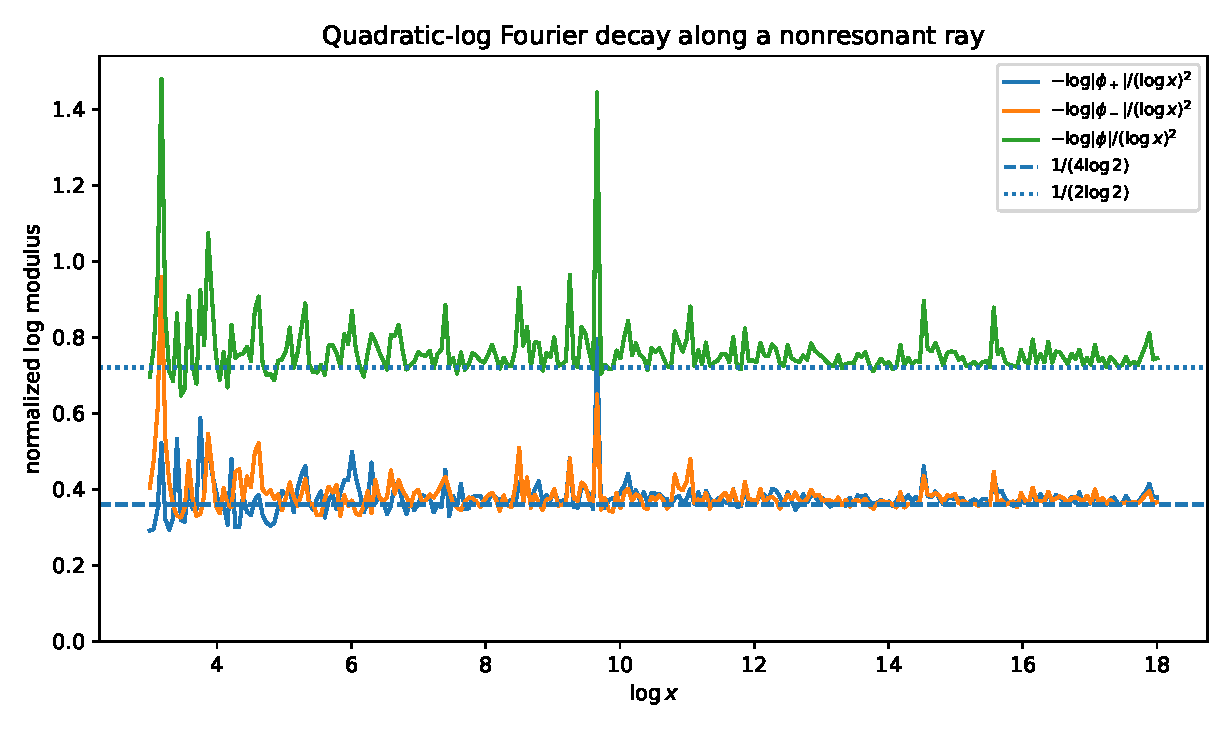
\includegraphics[width=0.92\textwidth]{fourier_decay.pdf}
\caption{Numerical values along $x=\e^L+\sqrt2$.  Exact zeros prevent a global two-sided
asymptotic, but away from resonances the normalized logarithms cluster near the density
predictions $1/(4\log2)$ for each factor and $1/(2\log2)$ for their product.}
\label{fig:fourier-decay}
\end{figure}

\begin{warning}
Equation~\eqref{eq:tm-Fourier-bound} is a rigorous upper bound, not a pointwise asymptotic
equivalence.  The real transforms have infinitely many zeros, so no finite lower bound can
hold on the whole real axis.
\end{warning}

\section{The exact zero divisor}
\label{sec:zeros}

Each factor $\sinc(z/2^n)$ has simple zeros at $z=\pi\ell2^n$, $\ell\in\Z\setminus\{0\}$.
The zeros of the full Rvachev transform are therefore $2\pi k$, $k\ne0$, with multiplicity
$1+\nu_2(k)$.  The automatic splitting gives a finer formula.

\begin{theorem}[Thue--Morse zero multiplicities]
\label{thm:zero-multiplicity}
Let $k\in\Z\setminus\{0\}$, put $N=1+\nu_2(k)$, and define
\begin{equation}
 S_N=\sum_{m=0}^{N-1}e_m.
 \label{eq:SN}
\end{equation}
Then the multiplicity of the zero $2\pi k$ in $\phi_\sigma$ is
\begin{equation}
 \boxed{\quad
 \operatorname{mult}_{2\pi k}(\phi_\sigma)
 =\frac{N+\sigma S_N}{2}.
 \quad}
 \label{eq:zero-multiplicity}
\end{equation}
Here
\begin{equation}
 S_{2r}=0,
 \qquad
 S_{2r+1}=e_r.
 \label{eq:prefix-exact}
\end{equation}
The two multiplicities add to $N$.
\end{theorem}

\begin{proof}
At $z=2\pi k$, the factor indexed by $n$ vanishes exactly when
$2^{n-1}\mid k$, equivalently $1\le n\le N$.  All such zeros are simple.  Counting the
selected indices among $1,\ldots,N$ gives
\[
 \sum_{m=0}^{N-1}\frac{1+\sigma e_m}{2}
 =\frac{N+\sigma S_N}{2}.
\]
The prefix identities follow by pairing $e_{2j}+e_{2j+1}=0$.
\end{proof}

\begin{corollary}[No equal compact convolution roots]
\label{cor:no-roots}
Neither $\mu_+$, $\mu_-$, nor the Rvachev law is a nontrivial $r$-fold convolution power
of a compactly supported probability measure for any integer $r\ge2$.
\end{corollary}

\begin{proof}
If $\mu=\nu^{*r}$ and both laws are compactly supported, their characteristic functions
extend to entire functions and $\phi_\mu=\phi_\nu^r$ on $\C$.  Every zero multiplicity of
$\phi_\mu$ must then be divisible by $r$.  The function $\phi_+$ has simple zeros at
$2\pi k$ for odd $k$.  The function $\phi_-$ has a simple zero at $4\pi$ (take $k=2$,
$N=2$).  Their product has the simple zeros at odd $k$.  Each case contradicts
divisibility.
\end{proof}

\begin{remark}
Thus the factorization $\mu_+*\mu_-=\mu_{\Up}$ is genuinely asymmetric: it does not arise
by extracting an equal convolution root.  The zero divisor records exactly which nested
dyadic zeros each automatic factor receives.
\end{remark}

\section{Mellin transform and the inherited natural boundary}
\label{sec:mellin}

Let
\begin{equation}
 K_\sigma(t)=\log\mathbb E\e^{tX_\sigma}
 =\sum_{m\ge0}a_m^\sigma h(t/2^{m+1}),
 \qquad h(t)=\log\frac{\sinh t}{t}.
 \label{eq:Ksigma}
\end{equation}
Set
\begin{equation}
 K_0=K_++K_-=
 \sum_{n\ge1}h(t/2^n),
 \qquad
 J=K_+-K_-=\sum_{m\ge0}e_mh(t/2^{m+1}).
 \label{eq:K0J}
\end{equation}

\begin{lemma}[Mellin transform of the uniform cumulant kernel]
\label{lem:mellin-h}
For $-2<\Re s<-1$,
\begin{equation}
 \Mell h(s):=\int_0^\infty h(t)t^{s-1}\dd t
 =\frac{\pi^{s+1}\zeta(-s)}{s\sin(\pi s/2)}
 =-2^{-s}\Gamma(s)\zeta(s+1).
 \label{eq:mellin-h}
\end{equation}
\end{lemma}

\begin{proof}
Euler's product for $\sinh$ is
\[
 \frac{\sinh t}{t}=\prod_{k\ge1}\left(1+\frac{t^2}{\pi^2k^2}\right).
\]
For $-2<\Re s<0$, integration by parts gives
\[
 \int_0^\infty y^{s-1}\log(1+y^2)\dd y
 =\frac{\pi}{s\sin(\pi s/2)}.
\]
In the smaller strip $\Re s<-1$, summation over $k$ is absolutely justified and yields the
first expression.  The second is the functional equation of the zeta function.
\end{proof}

\begin{theorem}[Mellin decomposition]
\label{thm:mellin-decomposition}
For $-2<\Re s<-1$,
\begin{align}
 \Mell K_0(s)
 &=-\frac{\Gamma(s)\zeta(s+1)}{1-2^s},
 \label{eq:mellin-K0}\\
 \Mell J(s)
 &=-\Gamma(s)\zeta(s+1)E(2^s),
 \label{eq:mellin-J}\\
 \Mell K_\sigma(s)
 &=-\frac12\Gamma(s)\zeta(s+1)
 \left(\frac1{1-2^s}+\sigma E(2^s)\right).
 \label{eq:mellin-Ksigma}
\end{align}
\end{theorem}

\begin{proof}
Mellin scaling gives
\(
 \Mell[h(t/2^n)](s)=2^{ns}\Mell h(s).
\)
Therefore
\[
 \sum_{n\ge1}2^{ns}=\frac{2^s}{1-2^s},
 \qquad
 \sum_{m\ge0}e_m2^{(m+1)s}=2^sE(2^s).
\]
Multiply by \eqref{eq:mellin-h}, and use
$K_\sigma=(K_0+\sigma J)/2$.
\end{proof}

\begin{corollary}[Natural boundary for the signed Mellin correction]
\label{cor:mellin-boundary}
The factor $E(2^s)$ is holomorphic for $\Re s<0$ and has the line $\Re s=0$ as a natural
boundary.  Consequently the meromorphic continuation of the right-hand side of
\eqref{eq:mellin-J} within $\Re s<0$ cannot be analytically continued through any open
segment of that line.
\end{corollary}

\begin{proof}
The map $s\mapsto2^s$ sends $\Re s<0$ to the unit disk and its boundary to the unit
circle.  By P\'olya--Carlson, $E$ has the unit circle as a natural boundary.  The remaining
factor $-\Gamma(s)\zeta(s+1)$ is meromorphic and is nonzero off a discrete set; it cannot
cancel singularities on every point of an open boundary segment.
\end{proof}

\begin{statusbox}{Novelty boundary}
The repository already contains a formal and semi-formal theory of the Thue--Morse natural
boundary and separate cyclotomic $q$-Fabius developments.  The new statement here is the
specific Mellin factorization \eqref{eq:mellin-Ksigma} for the scale-split laws.  The
natural-boundary conclusion is an application of occupied infrastructure, not claimed as
a new general boundary theorem.
\end{statusbox}

\section{Sharp logarithmic endpoint laws}
\label{sec:endpoint}

Let $A\subseteq\N_{\ge1}$ and suppose $A(N)=\delta N+\bigO(1)$.  Write
\begin{equation}
 D_A=R_A-X_A\ge0,
 \qquad
 G_A(\eps)=\Pr(D_A\le\eps).
 \label{eq:deficit}
\end{equation}
Because $2^{-n}-2^{-n}V_n$ is uniform on $[0,2^{1-n}]$, the deficit is a positive random
series
\begin{equation}
 D_A=\sum_{n\in A}2^{1-n}W_n,
 \qquad W_n\sim\operatorname{Unif}[0,1].
 \label{eq:deficit-series}
\end{equation}

\subsection{Laplace asymptotics}

\begin{theorem}[Deficit Laplace transform]
\label{thm:Laplace-asymptotic}
Under \eqref{eq:bounded-discrepancy}, as $t\to+\infty$,
\begin{equation}
 \log\mathbb E\e^{-tD_A}
 =-\frac{\delta}{2\log2}(\log t)^2+\bigO(\log t).
 \label{eq:Laplace-asymptotic}
\end{equation}
Equivalently,
\begin{equation}
 \log\mathbb E\e^{tX_A}
 =R_At-\frac{\delta}{2\log2}(\log t)^2+\bigO(\log t).
 \label{eq:mgf-edge}
\end{equation}
\end{theorem}

\begin{proof}
The logarithm of the Laplace transform is
\begin{equation}
 L_A(t)=\sum_{n\in A}\ell(2^{1-n}t),
 \qquad
 \ell(y)=\log\frac{1-\e^{-y}}{y}.
 \label{eq:ell-sum}
\end{equation}
For $y\ge1$, $\ell(y)=-\log y+\bigO(\e^{-y})$; for $0<y\le1$,
$\ell(y)=\bigO(y)$.  Put $N=\floor{\log_2t}$.  Terms with $n>N+O(1)$ contribute
$\bigO(1)$ in total, and the transition band contributes $\bigO(1)$.  Therefore
\begin{align}
 L_A(t)
 &=-\sum_{\substack{n\le N\\n\in A}}\log(2^{1-n}t)+\bigO(N)\\
 &=-A(N)\log t+\log2\sum_{\substack{n\le N\\n\in A}}(n-1)+\bigO(N).
 \label{eq:Laplace-count}
\end{align}
Use \eqref{eq:bounded-discrepancy}, \eqref{eq:weighted-count}, and
$N=(\log t)/(\log2)+\bigO(1)$ to obtain \eqref{eq:Laplace-asymptotic}.  Since
$\mathbb E\e^{tX_A}=\e^{R_At}\mathbb E\e^{-tD_A}$, the second formula follows.
\end{proof}

\subsection{Small-ball theorem}

\begin{theorem}[Sharp logarithmic small balls]
\label{thm:small-ball}
Under \eqref{eq:bounded-discrepancy}, as $\eps\downarrow0$,
\begin{equation}
 \boxed{\quad
 \log G_A(\eps)
 =-\frac{\delta}{2\log2}
 \left(\log\frac1\eps\right)^2
 +\bigO\!\left(
 \log\frac1\eps\,\log\log\frac1\eps
 \right).
 \quad}
 \label{eq:small-ball}
\end{equation}
\end{theorem}

\begin{proof}
Let $L=\log(1/\eps)$.  For the upper bound, exponential Markov with $t=1/\eps$ gives
\[
 G_A(\eps)
 =\Pr(\e^{-tD_A}\ge\e^{-t\eps})
 \le\e^{t\eps}\mathbb E\e^{-tD_A}.
\]
Apply \cref{thm:Laplace-asymptotic}; this yields
\[
 \log G_A(\eps)
 \le-\frac{\delta}{2\log2}L^2+\bigO(L).
\]

For the lower bound choose
$N=\ceil{\log_2(1/\eps)}+3$.  The deterministic tail after $N$ is at most
\(
 \sum_{n>N}2^{1-n}=2^{1-N}\le\eps/4.
\)
Let $M=A(N)$.  Require, for every selected $n\le N$,
\[
 2^{1-n}W_n\le\frac{3\eps}{4M}.
\]
Then the first $N$ terms total at most $3\eps/4$, and the tail completes an event contained
in $\{D_A\le\eps\}$.  For small $\eps$, all the displayed thresholds for $W_n$ lie below
one, so independence gives
\begin{align}
 \log G_A(\eps)
 &\ge\sum_{\substack{n\le N\\n\in A}}
 \log\left(\frac{3\eps}{4M\,2^{1-n}}\right)\\
 &=-ML-M\log(4M/3)+\log2
 \sum_{\substack{n\le N\\n\in A}}(n-1).
 \label{eq:small-ball-lower}
\end{align}
Now $M=\delta N+\bigO(1)$,
$\sum_{n\le N,n\in A}n=\delta N^2/2+\bigO(N)$, and
$N=L/\log2+\bigO(1)$.  The first and third terms combine to
$-\delta L^2/(2\log2)+\bigO(L)$, while $M\log M=\bigO(L\log L)$.  This proves the matching
lower bound and hence \eqref{eq:small-ball}.
\end{proof}

\begin{corollary}[Thue--Morse factor edges]
\label{cor:tm-small-ball}
For $\sigma=\pm1$,
\begin{equation}
 \log\Pr(R_\sigma-X_\sigma\le\eps)
 =-\frac1{4\log2}\left(\log\frac1\eps\right)^2
 +\bigO\!\left(\log\frac1\eps\log\log\frac1\eps\right).
 \label{eq:tm-small-ball}
\end{equation}
The same formula holds at the left endpoint by symmetry.
\end{corollary}

\begin{proof}
Use $\delta=1/2$ in \cref{thm:small-ball}.
\end{proof}

\begin{figure}[H]
\centering
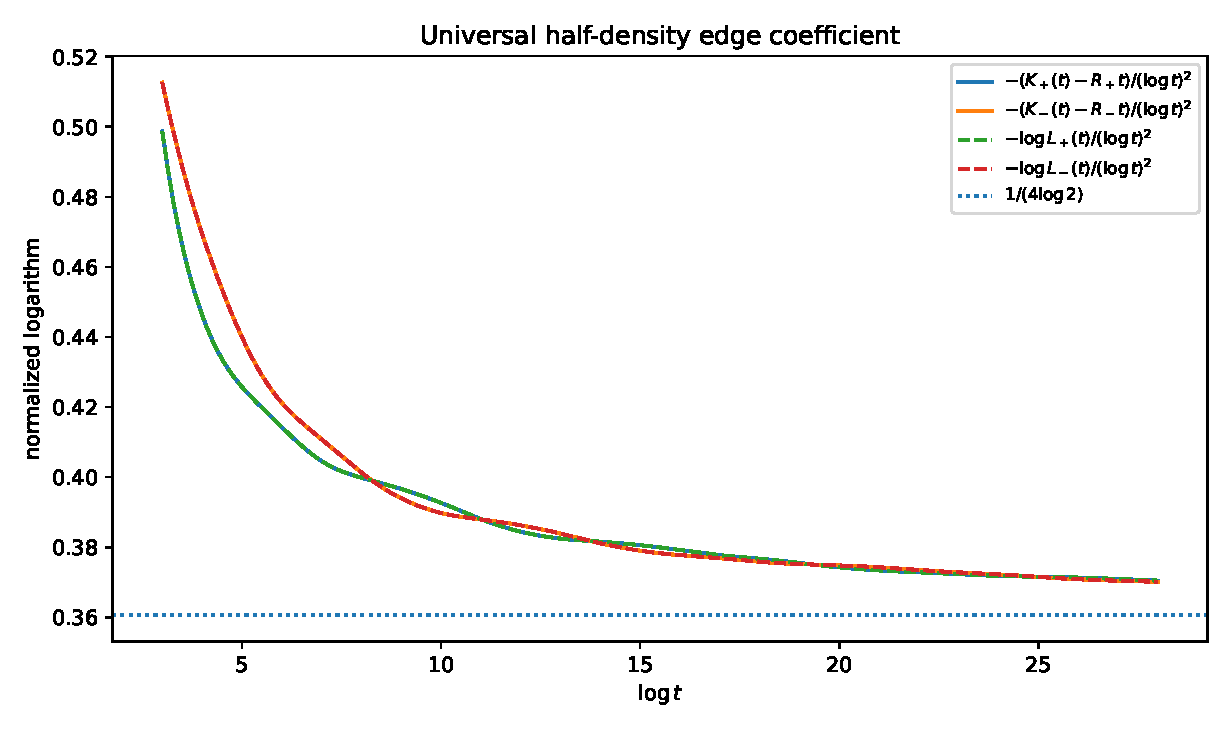
\includegraphics[width=0.92\textwidth]{laplace_mgf_asymptotics.pdf}
\caption{The support-reduced log-MGFs and deficit Laplace transforms approach the proved
coefficient $1/(4\log2)$.  The slow $1/\log t$ drift is expected from the unresolved
linear-logarithmic and automatic-hull terms.}
\label{fig:laplace}
\end{figure}

\section{Inverse-edge quantiles and Lambert-W coordinates}
\label{sec:inverse}

Let $Q_A(p)$ denote the quantile function of $X_A$.  We use the generalized inverse
$Q_A(p)=\inf\{x:\Pr(X_A\le x)\ge p\}$.  Under the hypotheses below the law has a
continuous density and full interval support, so its distribution function is continuous
and strictly increasing and the endpoint inversion is unambiguous.

\begin{theorem}[Inverse-edge scale]
\label{thm:inverse-edge}
Under \eqref{eq:bounded-discrepancy}, as $u\downarrow0$,
\begin{equation}
 \log\frac1{R_A-Q_A(1-u)}
 =\sqrt{\frac{2\log2}{\delta}\log\frac1u}
 +\bigO\!\left(\log\log\frac1u\right).
 \label{eq:inverse-edge}
\end{equation}
Equivalently,
\begin{equation}
 R_A-Q_A(1-u)
 =\exp\!\left[
 -\sqrt{\frac{2\log2}{\delta}\log\frac1u}
 +\bigO\!\left(\log\log\frac1u\right)
 \right].
 \label{eq:inverse-edge-exp}
\end{equation}
For the two Thue--Morse factors the square-root coefficient is
$2\sqrt{\log2}$.
\end{theorem}

\begin{proof}
Put $\eps=R_A-Q_A(1-u)$, so $u=G_A(\eps)$.  If
$Y=\log(1/u)$ and $L=\log(1/\eps)$, \cref{thm:small-ball} says
\[
 Y=\frac\delta{2\log2}L^2+\bigO(L\log L).
\]
Solving this quadratic-scale relation gives
$L=\sqrt{(2\log2/\delta)Y}+\bigO(\log Y)$, which is
\eqref{eq:inverse-edge}.
\end{proof}

The leading law is not itself a Lambert-$W$ formula; Lambert $W_{-1}$ appears after one
retains the derivative of the quadratic-log Laplace action.  Suppose heuristically that a
refined expansion along a stable symbolic phase has the form
\begin{equation}
 \log\mathbb E\e^{-tD_A}
 =-c(\log t)^2+d\log t+C+o(1),
 \qquad c=\frac\delta{2\log2}.
 \label{eq:refined-Laplace-heuristic}
\end{equation}
The saddle equation is then
\begin{equation}
 \eps t=2c\log t-d+o(1).
 \label{eq:saddle-equation}
\end{equation}
Ignoring the $o(1)$ term yields the explicit chart
\begin{equation}
 \log t
 =-W_{-1}\!\left(-\frac{\eps}{2c}\e^{d/(2c)}\right)-\frac d{2c}.
 \label{eq:Lambert-chart}
\end{equation}
For the ordinary dyadic law, periodic log-scale corrections can be inserted into such
charts.  For the automatic factors, \cref{id:shift-cocycle} suggests that $d$ and $C$ are
not scalar periodic functions but observables on the Thue--Morse shift hull.  This is the
basis of \cref{conj:symbolic-saddle}.

\section{Finite dyadic spline approximants}
\label{sec:splines}

The infinite factors admit exact finite-stage approximants with dyadic knots and rational
coefficients.  Let
\begin{equation}
 A_{\sigma,N}=A_\sigma\cap[1,N],
 \qquad m_{\sigma,N}=|A_{\sigma,N}|,
 \qquad R_{\sigma,N}=\sum_{n\in A_{\sigma,N}}2^{-n}.
 \label{eq:finite-selector}
\end{equation}
The finite sum $X_{\sigma,N}$ is a convolution of $m_{\sigma,N}$ uniform densities and is
a nonuniform cardinal box spline.

\begin{proposition}[Explicit finite spline]
\label{prop:finite-spline}
For $m=m_{\sigma,N}\ge1$, the density of $X_{\sigma,N}$ is
\begin{equation}
 u_{\sigma,N}(x)
 =\frac{1}{(m-1)!\prod_{n\in A_{\sigma,N}}2^{1-n}}
 \sum_{S\subseteq A_{\sigma,N}}(-1)^{|S|}
 \left(x+R_{\sigma,N}-\sum_{n\in S}2^{1-n}\right)_+^{m-1}.
 \label{eq:finite-spline}
\end{equation}
It is piecewise polynomial of degree $m-1$, with knots on the lattice $2^{1-N}\Z$.
Moreover $X_{\sigma,N}\to X_\sigma$ almost surely and uniformly under the canonical
coupling, with
\begin{equation}
 |X_\sigma-X_{\sigma,N}|
 \le\sum_{n>N}2^{-n}=2^{-N}.
 \label{eq:coupling-error}
\end{equation}
Hence the distribution functions satisfy the certified quantile brackets
\begin{equation}
 Q_{\sigma,N}(p)-2^{-N}\le Q_\sigma(p)
 \le Q_{\sigma,N}(p)+2^{-N}.
 \label{eq:quantile-bracket}
\end{equation}
\end{proposition}

\begin{proof}
Shift each uniform interval $[-2^{-n},2^{-n}]$ to $[0,2^{1-n}]$ and apply the standard
inclusion--exclusion formula for the density of a sum of independent nonidentical uniform
variables.  Shifting back gives \eqref{eq:finite-spline}.  Every endpoint is dyadic with
denominator at most $2^{N-1}$, proving the knot statement.  The tail bound is deterministic,
and the quantile bracket follows from the $W_\infty$ coupling estimate.
\end{proof}

\begin{algorithm}[Certified evaluation]
For fixed $N$, sort the dyadic knots in \eqref{eq:finite-spline}, aggregate equal subset
sums by dynamic programming rather than enumerating all $2^m$ subsets, and evaluate the
appropriate polynomial piece using exact rational arithmetic.  Integrating once gives an
exact rational-piece CDF; monotone bisection plus \eqref{eq:quantile-bracket} then gives a
certified inverse value.  The automatic recursion can reuse tables between $N$, $2N$, and
adjacent shift states.
\end{algorithm}

\section{Numerical experiments}
\label{sec:numerics}

The companion script \texttt{thue\_morse\_factors.py} uses 80-decimal mpmath arithmetic
for products and transforms, and a deterministic NumPy generator for the illustrative
density plot.  It writes all plotted samples and checks to CSV or JSON.  The principal
checks are:
\begin{enumerate}
\item agreement of the series and product definitions of $E(1/2)$ to 60 displayed digits;
\item $R_++R_-=1$ to working precision;
\item the complex product identity $\phi_+\phi_-=\widehat\Up$ with residual
$2.2\times10^{-81}$ at the test point;
\item both q-Mahler identities with residuals below $5\times10^{-81}$;
\item the Mellin formula \eqref{eq:mellin-h} at $s=-3/2$ and at
$s=-1.4+0.3\ii$, with numerical integration errors about $10^{-22}$ and $10^{-27}$;
\item the exact zero multiplicity table for $1\le k\le32$;
\item convergence of the normalized edge logarithms to $1/(4\log2)$.
\end{enumerate}

\begin{figure}[H]
\centering
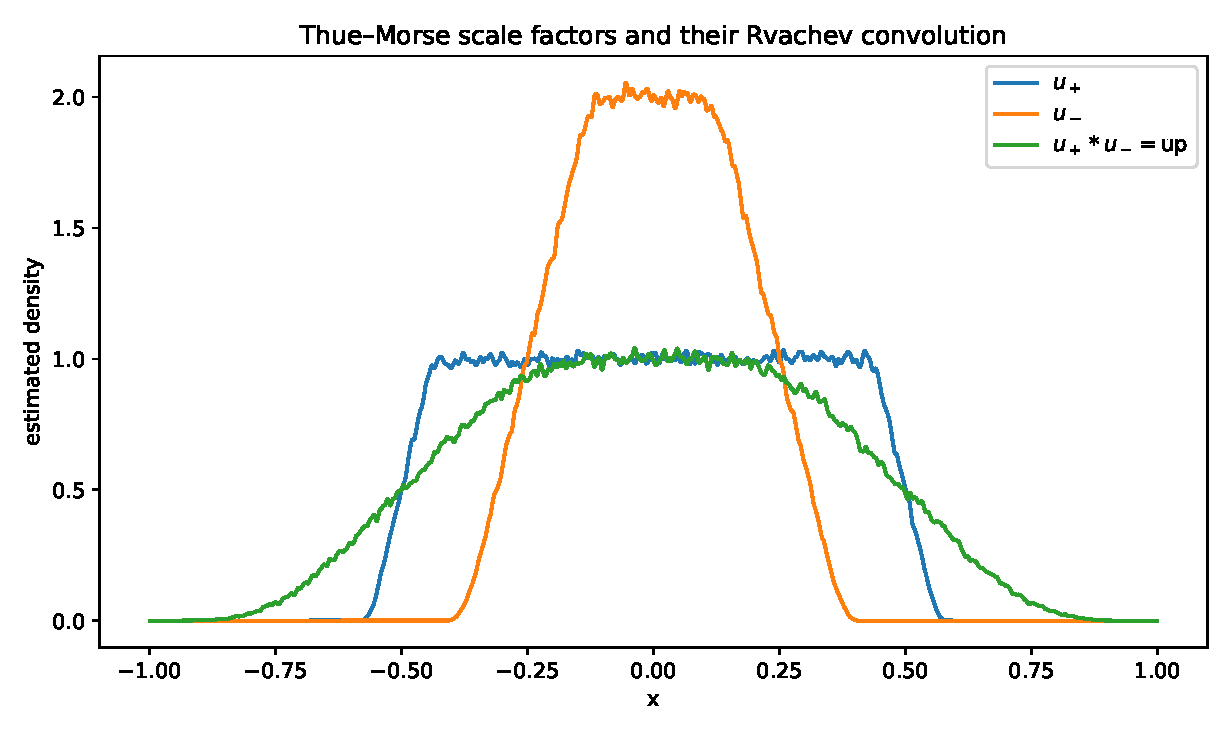
\includegraphics[width=0.92\textwidth]{factor_densities.pdf}
\caption{Monte Carlo illustration using $500{,}000$ coupled samples and 45 dyadic scales.
The exact plateaux are already conspicuous: height $1$ for $u_+$ and height $2$ for $u_-$.
The green curve is the coupled sum, whose exact law is $\Up$.}
\label{fig:density-factors}
\end{figure}

The histogram convolution check has $L^1$ discrepancy about $1.49\times10^{-2}$; this is
consistent with sampling, binning, smoothing, and finite-tail error and is not used as a
proof.  The analytical identity is exact.

\section{General base and automatic-selector extension}
\label{sec:generalization}

The leading analytic mechanism is not special to base two.  Let $b>1$ and
\begin{equation}
 X_{A,b}=\sum_{n\in A}b^{-n}V_n,
 \qquad
 R_{A,b}=\sum_{n\in A}b^{-n}.
 \label{eq:base-b}
\end{equation}

\begin{theorem}[Base-$b$ selector universality]
\label{thm:base-b}
If $A(N)=\delta N+\bigO(1)$, then
\begin{align}
 \log|\phi_{A,b}(x)|
 &\le-\frac\delta{2\log b}(\log|x|)^2+\bigO(\log|x|),
 \label{eq:base-b-Fourier}\\
 \log\mathbb E\e^{-t(R_{A,b}-X_{A,b})}
 &=-\frac\delta{2\log b}(\log t)^2+\bigO(\log t),
 \label{eq:base-b-Laplace}\\
 \log\Pr(R_{A,b}-X_{A,b}\le\eps)
 &=-\frac\delta{2\log b}\left(\log\frac1\eps\right)^2
 +\bigO\!\left(\log\frac1\eps\log\log\frac1\eps\right).
 \label{eq:base-b-small}
\end{align}
In particular $X_{A,b}$ has a $C^\infty$ density whenever $\delta>0$.
\end{theorem}

\begin{proof}
Repeat the proofs of \cref{thm:selector-Fourier,thm:Laplace-asymptotic,thm:small-ball},
replacing $2$ by $b$.  The quadratic weighted count is unchanged, while
$N\sim(\log x)/(\log b)$ supplies the new denominator.
\end{proof}

Balanced automatic and morphic selectors are especially promising because their counting
functions often have bounded or explicitly controlled discrepancy and their generating
functions satisfy finite Mahler systems.  The Thue--Morse pair is the simplest nonperiodic
example where positivity, complementarity, exact support algebra, and a natural boundary
occur simultaneously.

\section{Conjectures and frontier problems}
\label{sec:conjectures}

The following statements are deliberately separated from the proved results.

\begin{conjecture}[Symbolic-hull saddle expansion]
\label{conj:symbolic-saddle}
There exist continuous observables $B,C,\ldots$ on the two-sided Thue--Morse substitution
hull $\Omega_{\rm TM}$ such that, after associating to $t$ the shift state selected by
$\floor{\log_2t}$,
\begin{equation}
 \log\mathbb E\e^{-tD_\sigma}
 =-\frac{(\log t)^2}{4\log2}
 +B(\omega_t)\log t+C(\omega_t)
 +\sum_{j\ge1}\frac{C_j(\omega_t)}{(\log t)^j}
 \label{eq:symbolic-saddle-conj}
\end{equation}
holds in an appropriate asymptotic or transasymptotic sense.  Ordinary log-periodicity is
recovered when the selector is periodic; Thue--Morse replaces the circle phase by a
minimal symbolic dynamical system.
\end{conjecture}

\begin{conjecture}[Automatic Lambert atlas]
\label{conj:Lambert-atlas}
The endpoint density and quantile admit uniformly overlapping charts of the form
\eqref{eq:Lambert-chart}, with chart parameters continuous on $\Omega_{\rm TM}$.  Branch
switches are governed by the substitution map, and no finite Fourier series in
$\log_2\eps$ can represent the complete correction.
\end{conjecture}

\begin{conjecture}[Compact spectral-factor rigidity]
\label{conj:rigidity}
Let $\nu_1,\nu_2$ be centered symmetric compactly supported probability measures with
entire characteristic functions of Cartwright class, and suppose
$\nu_1*\nu_2=\mu_{\Up}$.  Under the additional condition that every zero of each factor
lies in the Rvachev zero set and both quotients have completely regular growth, the
factorization is induced by assigning whole dyadic sinc factors, up to a finite
B-spline factor and interchange of the two laws.
\end{conjecture}

\begin{remark}
The zero condition is essential.  General positive-definite entire spectral factorizations
may redistribute growth without visibly grouping the canonical factors.  The conjecture
is intended as a precise starting point, not as a claim that arbitrary convolution factors
are already classified.
\end{remark}

\begin{conjecture}[Jacobi substitution limit]
\label{conj:Jacobi}
After normalization to $[-1,1]$, the Jacobi parameters $\beta_n^\pm$ in
\eqref{eq:Jacobi} possess a compact limit set generated by a finite-dimensional
renormalization over the Thue--Morse hull.  The paired sequences are related by the
involution induced by $e_{2m+1}=-e_m$.
\end{conjecture}

\begin{conjecture}[Matching local Fourier envelope]
\label{conj:Fourier-envelope}
For each sign there exists a fixed $C>0$ such that
\begin{equation}
 \sup_{y\in[x,x+C]}\log|\phi_\sigma(y)|
 =-\frac1{4\log2}(\log x)^2+\bigO(\log x).
 \label{eq:local-envelope}
\end{equation}
This would complement the one-sided global bound by showing that no additional quadratic
loss persists after a bounded local avoidance of zeros.
\end{conjecture}

\begin{problem}[Arithmetic of selected dyadic values]
Determine denominator bounds and integrality normalizations for
$u_\pm(r/2^N)$ and their derivatives.  Finite-stage values are rational by
\eqref{eq:finite-spline}, but passage to the $C^\infty$ limit couples the lacunary Mahler
values $E(2^{-2r})$ to the dyadic spline arithmetic.  It is unclear whether analogues of
the known Fabius integer sequences survive.
\end{problem}

\begin{problem}[Natural-boundary resurgence]
Develop a contour calculus for \eqref{eq:mellin-Ksigma} that does not cross
$\Re s=0$.  One possible replacement for a residue lattice is approximation by rational
Thue--Morse blocks, followed by a limit in which finite pole lattices condense to the
natural boundary.  Quantify which edge coefficients stabilize before condensation.
\end{problem}

\begin{problem}[More than two colors]
Partition the scales by a balanced $k$-automatic word into $r>2$ classes.  Classify when
every class has positive density and hence a smooth density, derive the matrix Mahler
system for the $r$ characteristic factors, and determine which substitutions produce
exact plateaux or nested support coincidences analogous to \cref{thm:exact-plateaux}.
\end{problem}

\section{Formalization blueprint}
\label{sec:lean}

A Lean development can be split into largely independent layers.

\paragraph{Combinatorics.}
Formalize $e_n=(-1)^{\operatorname{popcount}(n)}$, the recurrences
$e_{2n}=e_n$, $e_{2n+1}=-e_n$, prefix sums \eqref{eq:prefix-exact}, selector counts, and
weighted-count summation by parts.  Much of the natural-boundary infrastructure already
exists in the repository and should be reused rather than duplicated.

\paragraph{Probability and convolution.}
Construct the finite independent uniform sums first.  Prove deterministic Cauchy bounds
for the tails and pass to the limit in distribution.  Establish
\eqref{eq:main-factorization} at the finite level, then use weak convergence.  Support
radii reduce to absolutely convergent geometric sums.

\paragraph{Fourier analysis.}
Prove local uniform convergence of the entire products and the bound
$|\sinc x|\le\min(1,1/|x|)$.  The weighted selector count then gives rapid decay.  Existing
Fourier inversion lemmas can convert weighted $L^1$ bounds to $C^\infty$ densities.

\paragraph{Plateaux.}
The dominant-uniform lemma is elementary measure theory and should be formalized before
smoothness: the constant region follows from interval containment.  Infinite-order
flatness then uses the smoothness result and differentiation of convolution.

\paragraph{Moments.}
Bernoulli cumulants may be handled first as formal power series.  The selector generating
function \eqref{eq:selector-generating} is algebraic once $E(q)$ is available.  Bell
recurrences avoid committing to a large combinatorial-polynomial library.

\paragraph{Endpoint asymptotics.}
Formalize the logarithmic Laplace estimate using explicit inequalities for
$\ell(y)=\log((1-\e^{-y})/y)$ on $(0,1]$ and $[1,\infty)$.  The small-ball lower bound is a
finite product event plus a deterministic tail estimate; it does not require a deep
Tauberian theorem.  This makes \cref{thm:small-ball} unusually suitable for formal proof.

\section{Conclusions}

Partitioning the uniform scales, rather than manipulating the completed Rvachev transform,
opens a distinct structural direction.  The Thue--Morse word produces two genuine smooth
compactly supported laws whose convolution is $\Up$, whose supports are measured by a
Mahler product, and whose exact plateaux remember the first automatic digits.  Their
cumulants combine Bernoulli numbers with $E(q^{2r})$, their moments pass through Bell
polynomials, and their Legendre data are finite consequences of the same q-values.  At the
spectral level, finite Thue--Morse prefix sums split every nested zero multiplicity.  At the
edge, only selector density controls the leading quadratic logarithm, while the exact
automatic order is expected to reappear in the next symbolic-hull layer.

The strongest proved frontier result is perhaps the combination of positivity and
nonperiodicity: natural-boundary behavior is not confined to a formal signed series, but is
embedded inside a pair of nonnegative $C^\infty$ probability densities with an exact
convolutional relation to the classical Fabius/Rvachev object.  This gives a concrete test
case where automatic sequences, q-Mahler equations, compactly supported harmonic analysis,
small deviations, Lambert-$W$ inversion, and orthogonal-polynomial data can be studied in a
single rigorously connected model.

\appendix

\section{Additional exact identities}

\subsection{Weighted Thue--Morse prefixes}
Let
\begin{equation}
 T_N=\sum_{m=0}^{N-1}m e_m.
 \label{eq:weighted-prefix-def}
\end{equation}
Pairing even and odd indices gives
\begin{align}
 T_{2M}
 &=\sum_{r=0}^{M-1}\bigl(2r e_{2r}+(2r+1)e_{2r+1}\bigr)
 =-\sum_{r=0}^{M-1}e_r=-S_M,
 \label{eq:T-even}\\
 T_{2M+1}
 &=T_{2M}+2M e_{2M}
 =-S_M+2Me_M.
 \label{eq:T-odd}
\end{align}
A version shifted by one index controls exact linear-logarithmic terms in finite truncations
of $K_+-K_-$.  These formulas are one reason to expect a bounded-state symbolic correction
rather than an arbitrary error term.

\subsection{Complementary variance check}
Cumulants add under convolution, so
\begin{equation}
 \kappa_{2r}^++\kappa_{2r}^-
 =\frac{2^{2r-1}B_{2r}}r\frac{2^{-2r}}{1-2^{-2r}},
 \label{eq:cumulant-sum}
\end{equation}
which is exactly the known cumulant of the Rvachev law.  For $r=1$,
\begin{equation}
 \Var(X_+)+\Var(X_-)=\frac19,
 \label{eq:variance-sum}
\end{equation}
consistent with $\sum_{n\ge1}4^{-n}/3=1/9$.

\section{Reproducibility inventory}

The archive contains:
\begin{itemize}
\item \texttt{automatic\_scale\_factorizations.tex}: this source;
\item \texttt{automatic\_scale\_factorizations.pdf}: the compiled report;
\item \texttt{thue\_morse\_factors.py}: fully commented experiments;
\item \texttt{requirements.txt}: Python dependency list;
\item \texttt{figures/*.pdf} and \texttt{figures/*.png}: generated plots;
\item \texttt{data/cumulants\_and\_moments.csv};
\item \texttt{data/zero\_multiplicities.csv};
\item \texttt{data/mellin\_checks.csv};
\item \texttt{data/fourier\_decay.csv};
\item \texttt{data/laplace\_mgf\_asymptotics.csv};
\item \texttt{data/density\_histograms.csv};
\item \texttt{data/numerical\_summary.json};
\item \texttt{NOVELTY\_AUDIT.md} and \texttt{README.txt}.
\end{itemize}

\begin{thebibliography}{99}

\bibitem{Fabius1966}
J.~Fabius,
\newblock A probabilistic example of a nowhere analytic $C^\infty$-function,
\newblock \emph{Z. Wahrscheinlichkeitstheorie verw. Gebiete} \textbf{5} (1966), 173--174.

\bibitem{Arias1982}
J.~Arias de Reyna,
\newblock Definici\'on y estudio de una funci\'on indefinidamente diferenciable de soporte compacto,
\newblock \emph{Rev. Real Acad. Cienc. Exact. F\'is. Natur. Madrid} \textbf{76} (1982), 21--38.

\bibitem{Arias2017Compact}
J.~Arias de Reyna,
\newblock An infinitely differentiable function with compact support: definition and properties,
\newblock English translation of the 1982 paper, arXiv:1702.05442, 2017.

\bibitem{AriasArithmetic}
J.~Arias de Reyna,
\newblock Arithmetic of the Fabius function,
\newblock arXiv:1702.06487, 2017.

\bibitem{AlloucheMendesFrance2008}
J.-P.~Allouche and M.~Mend\`es France,
\newblock Euler, Pisot, Prouhet--Thue--Morse, Wallis and the duplication of sines,
\newblock \emph{Monatsh. Math.} \textbf{155} (2008), 301--315.

\bibitem{AlloucheShallit}
J.-P.~Allouche and J.~Shallit,
\newblock \emph{Automatic Sequences: Theory, Applications, Generalizations},
\newblock Cambridge University Press, 2003.

\bibitem{Carlson1921}
F.~Carlson,
\newblock \"Uber Potenzreihen mit ganzzahligen Koeffizienten,
\newblock \emph{Math. Z.} \textbf{9} (1921), 1--13.

\bibitem{JessenWintner1935}
B.~Jessen and A.~Wintner,
\newblock Distribution functions and the Riemann zeta function,
\newblock \emph{Trans. Amer. Math. Soc.} \textbf{38} (1935), 48--88.

\bibitem{DynRon1995}
N.~Dyn and A.~Ron,
\newblock Multiresolution analysis by infinitely differentiable compactly supported functions,
\newblock \emph{Appl. Comput. Harmon. Anal.} \textbf{2} (1995), 15--20.

\bibitem{ProveIt}
V.~Reshetnikov,
\newblock \repo, \path{Analysis/FabiusFunction/docs}, GitHub research corpus,
\newblock revision audited 30 August 2026.

\bibitem{RepresentationFrontiers}
\newblock \emph{Representation Frontiers for the Fabius--Rvachev System},
\newblock consolidated volume in the \repo\ semi-formalized research-frontier corpus,
28 August 2026.

\bibitem{CyclotomicReport}
\newblock \emph{Cyclotomic Blow-Ups and Natural Boundaries for the q-Fabius--Rvachev Sinc Product},
\newblock in the \repo\ semi-formalized research-frontier corpus, 30 August 2026.

\bibitem{DivisorReport}
\newblock \emph{Reciprocal-Integer Convolution Divisors of the Rvachev Law},
\newblock in the \repo\ semi-formalized research-frontier corpus, 30 August 2026.

\end{thebibliography}

\end{document}
